
\begin{lstlisting}[language=matlab, caption=Programa de procesamiento de datos provenientes de tarjeta PCI-6221]

%Variables iniciales
L = length(ACL1);
Fs = 200;
Reg = L/Fs
deltat = 1/Reg
count = 0;
time = [];

%Se convierten datos de string a double para poder graficarlos
%A = str2double(ACL1(1:5000));
A = str2double(ACL1);
B = str2double(ACL2);
C = str2double(ACL3);
time = str2double(TIME);

%Eliminacion de offset
A = A - mean(A);
B = B - mean(B);
C = C - mean(C);

%Kinemetrics FBA-11 1g = 2.5V
A = A*1.96; %Para convertir a m/s^2> (9.8m/s^2)/(2.5V)
B = B*1.96;
C = C*1.96;

%Generacion de graficas en tiempo
plot(time, A)
grid on;
hold on;
plot(time, B)
plot(time, C)
legend('Eje X','Eje Z', 'Eje Y')
% Add axis labels
ylabel('Amplitud (m/s^2)')
xlabel('Tiempo (s)')


%Calculo de la FFT y graficas del espectro en frecuencia
NFFT = 2^nextpow2(L);
Yout1 = fft(A,NFFT)/L;
Yout2 = fft(B,NFFT)/L;
Yout3 = fft(C,NFFT)/L;
fout = Fs/2*linspace(0,1,NFFT/2+1);
figure;
plot(fout,2*abs(Yout1(1:NFFT/2+1)))
hold on;
plot(fout,2*abs(Yout2(1:NFFT/2+1)))
plot(fout,2*abs(Yout3(1:NFFT/2+1)))

legend('Espectro eje X','Espectro eje Z', 'Espectro eje Y')
ylabel('Amplitud')
xlabel('Frecuencia (Hz)')

clearvars L;

\end{lstlisting}

    //Generacion de variables iniciales
    \begin{lstlisting}[language=java, caption=Programa de procesamiento para generación de archivos .csv en NodeRED]
        
        var xArray = msg.payload["esp32/x"]["x"];
        var yArray = msg.payload["esp32/y"]["y"];
        var zArray = msg.payload["esp32/z"]["z"];
        var temp = msg.payload["esp32/temp"];
        var hum =  msg.payload["esp32/hum"];
        var yaw =  msg.payload["esp32/inc_y"];
        var pitch =  msg.payload["esp32/inc_p"];
        var roll =  msg.payload["esp32/inc_r"];
        var time = msg.payload["esp32/timestamp"];
        
        //FECHA Y HORA DE RECEPCION DEL REGISTRO
        var date = new Date();
        var path = "C:\\Users\\jatov\\Documents\\Universidad\\TEG\\Pruebas_DatosAceleracion\\DatosACL_P1";
        var filename = path + "\\" + "data_" + date.getFullYear() + "_" + (date.getMonth()+1) + "_" + date.getDate() + "_" + date.getHours() + "_" + date.getMinutes() + "_" + date.getSeconds() + ".csv";
        
        if (!Array.isArray(xArray) || !Array.isArray(yArray) || !Array.isArray(zArray)) {
            node.error("msg.payload.x, msg.payload.y, and msg.payload.z must be arrays");
            return;
        }
        
        var output = [];
        
        for (var i = 0; i < xArray.length; i++) {
            if(i == 0){
                output.push({x: xArray[i], y: yArray[i], z: zArray[i], temp: temp, hum: hum, yaw: yaw, pitch: pitch, roll: roll, time: time});
            }
            output.push({x: xArray[i], y: yArray[i], z: zArray[i]});
        }
        
        
        //return {payload:output, filename:filename};
        
        msg.payload = output;
        msg.filename = filename;
        return msg;

\end{lstlisting}

\begin{figure}[H]
    \centering
    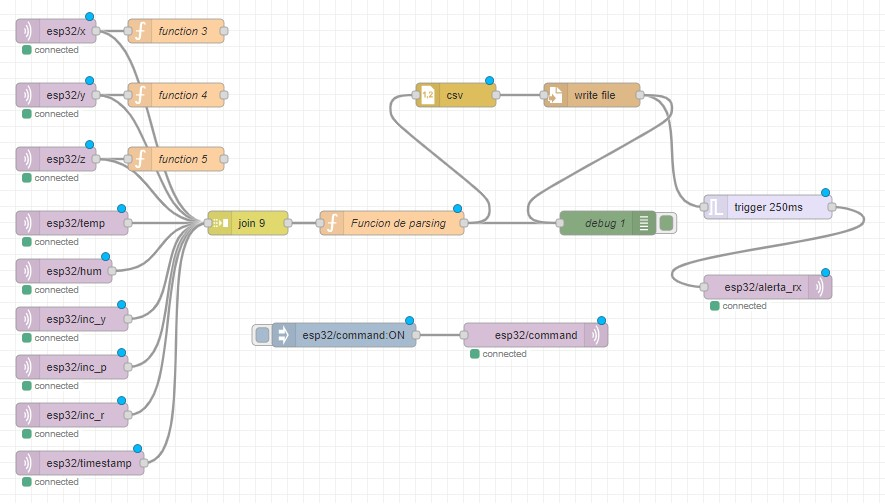
\includegraphics[width = \textwidth]{imagenes/cap3_resultados/Anexos/FlujoNodeRED.jpg}
    \caption{Flujo de nodered diseñado para el formateo de los datos provenientes del sistema receptor en la estación base.}
    \label{fig:flujonodered}
\end{figure}